\chapter{Model Driven Architecture (MDA)}
	\section{Origins}
		\begin{itemize}
			\item There are so many (not necessarily interoperable) technologies
			\item These evolve and get obsolete very quickly
		\end{itemize}
		$ \Longrightarrow $ desire to have ones business logic (processes, rules, \ldots) to be as independent as possible from any one technology (\textit{future-proof} business logic)\Biglb
		
	\section{Terminology}
		\subsection{Architecture}
			specification of the parts and connectors of the system and the rules for the interactions of the parts using the connectors.
			
		\subsection{Platform}
			Set of subsystems/technologies that provide a coherent	set of functionality through interfaces and specified usage	patterns.\\
			Any subsystem that depends on the platform can use it without concern for the details of how the functionality provided by the platform is implemented.
			
		\subsection{Implementation}
			A specification which provides all the	information needed to construct a system and to put it into
			operation.\Biglb
			
			
	\section{MDA Models}
		\subsection{Computation independent model (CIM)}
			\begin{itemize}
				\item a.k.a. \textit{domain model} or \textit{business model}
				\item focuses on the system and its environment; details of the structure of the system are hidden or undetermined
				\item specified using a vocabulary that is familiar to the practitioners of the domain in question
				\item may hide information about the use of	automated data processing systems
			\end{itemize}
		
		\subsection{Platform Independent Model (PIM)}
			Exhibits platform independence and is suitable for use with a number of different platforms of similar type.
			
		\begin{figure}[h!]
			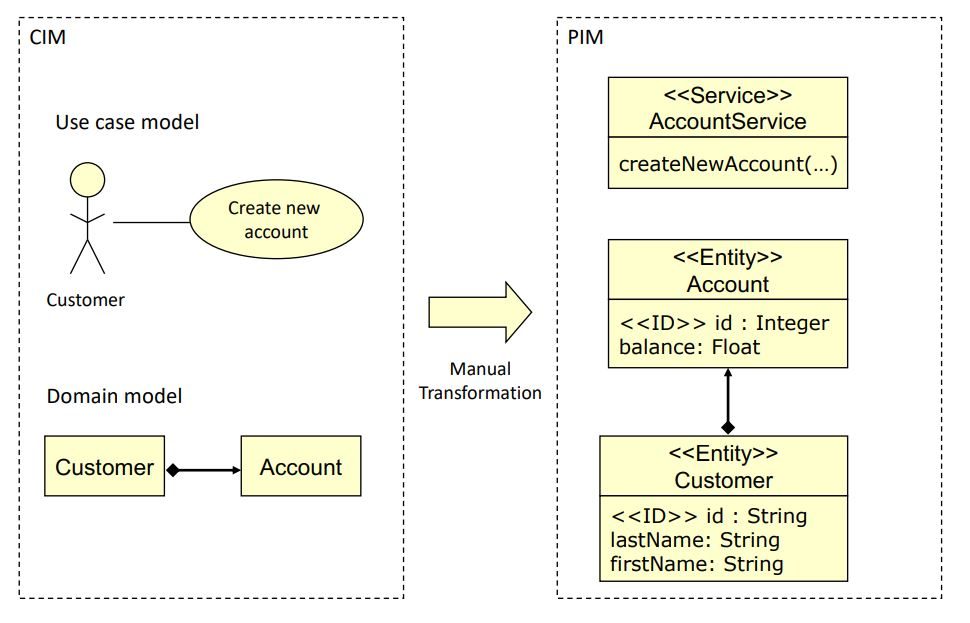
\includegraphics[scale=0.5]{res/cim-to-pim.jpg}
			\caption{How to convert a CIM to a PIM}
		\end{figure}
			
		\subsection{Platform Specific Model (PSM)}
			 Combines the specifications in the PIM with the details that specify how that system uses a particular type of platform.
			 
		\begin{figure}[h!]
			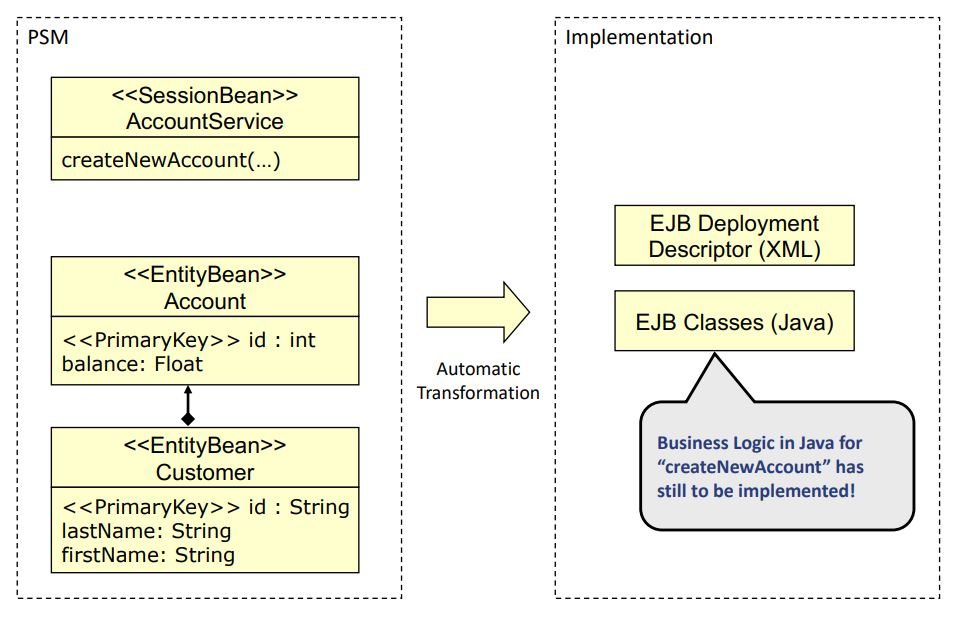
\includegraphics[scale=0.5]{res/psm-to-impl.jpg}
			\caption{Conversion from a PSM to an implementation}
		\end{figure}	 
			 
			 
		\subsection{Platform Model (PM)}
			Provides a set of technical concepts, representing the different kinds of parts that make up a
			platform and the services provided.\\
			Influences the way a PIM is mapped to a PSM.\Biglb			
			
		
	\section{Model transformation}
		This is the process of converting one model to another model of the same system. It is done by a process called \textbf{mapping}. An MDA mapping is a set of specifications for transformation of a PIM into a PSM for a particular platform. The platform model will determine the nature of the mapping.
		\begin{figure}[h!]
			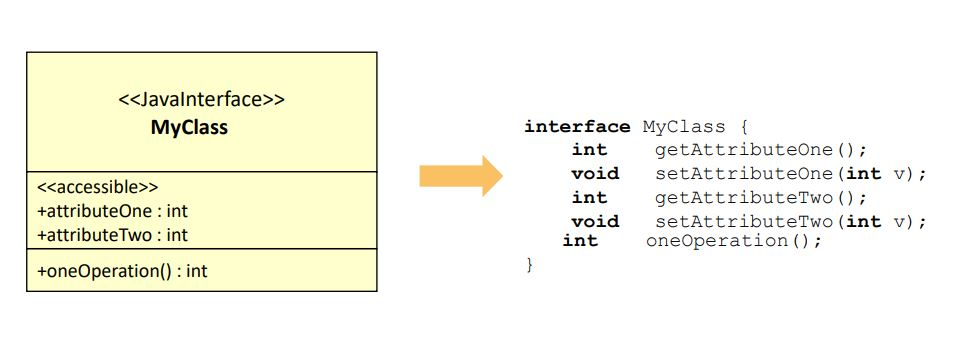
\includegraphics[scale=0.6]{res/mda-model-to-code-transformation.JPG}
			\caption{Model-to-code transformation -- an example for a mapping}
		\end{figure}
		
		\pagebreak
		
		\subsection{The MDA Pattern}
			The MDA pattern includes at least
			\begin{itemize}
				\item a PIM
				\item a PM
				\item a Transformation
				\item a PSM
			\end{itemize}
			\begin{figure}[h!]
				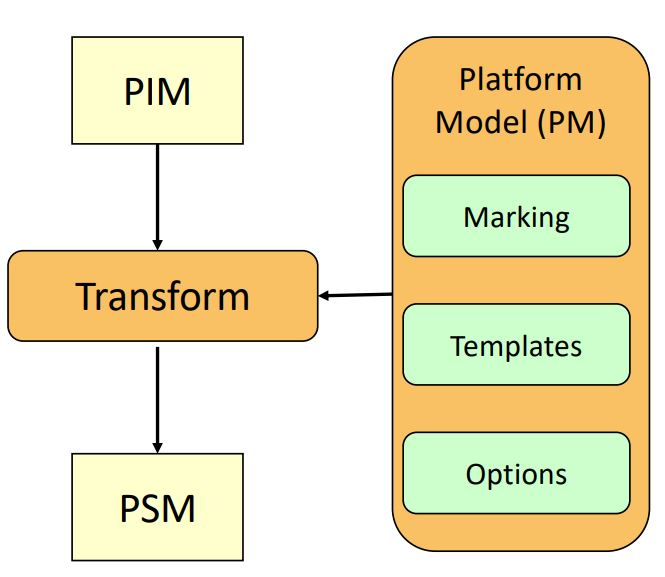
\includegraphics[scale=0.5]{res/mda-pattern.jpg}
				\caption{The MDA pattern (minimal form)}
			\end{figure}
			As shown in the figure, the PM influences the nature of the mapping. The PM does this through three concepts (first two described more elaborately in a later section):
			\begin{enumerate}
				\item Marking
				\item Transformation Templates
				\item Options: Adjust the transformation globally (similar to compiler options)\\
			\end{enumerate}
		
		
		\subsection{Mapping Concepts}
			\subsubsection{Metamodel Mapping}
				mapping gives rules and/or algorithms how types of the PIM metamodel are to be transformed to
				types of the PSM metamodel. Not applicable if PSM has no metamodel specified, e.g. in Model-to-Code transformations, where the PSM is Code. \Biglb
		
			\subsubsection{Marking}
				A mark represents a concept in the PSM, which can be applied to an element of the PIM to indicate how that element is to be transformed: \\
				if more than one PSM-alternative for something in the PIM exists, the mark indicates which alternative should be taken.\\Also,	different platform mappings may require different markings. \\
				Example from the lecture: In J2EE, there are two types of EJBs. Marking defines which one to use.
				
			\subsubsection{Transformation Templates}
				Parameterized models that specify particular kinds of transformations (a bit like design patterns). Typically creates groups of elements out of one element in the PIM.
				\begin{figure}[h!]
					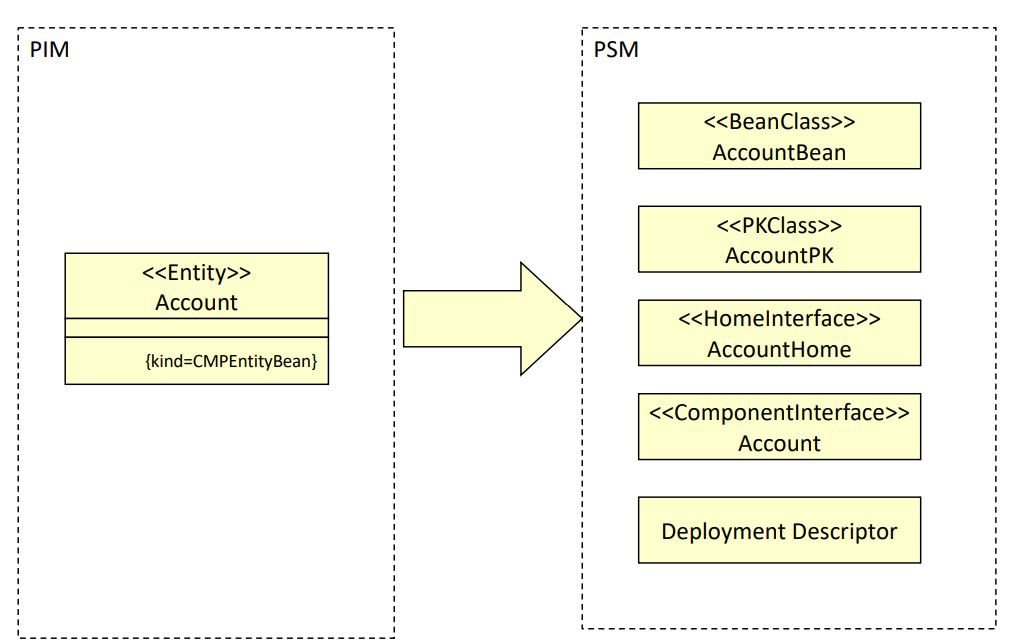
\includegraphics[scale=0.4]{res/mda-trans-templ.jpg}
					\caption{Example for a Transformation template}
				\end{figure}  	
		
		
			\subsubsection{Multi-staged Transformation}
				$ = $ Applying MDA Pattern in a cascade. The MDA pattern can (and usually has to) be  applied several times in succession; the output PSM from one iteration will then become a PIM for the next one\\ $ \Longrightarrow $ PIM and PSM are relative concepts,	they depend on the platform in use
				
			\subsubsection{Multi-platform Transformation}
				Many systems are (can be) built on more than one platform. Multi-platform Transformation means using different PMs to transform a PIM into different PSMs with parts of the system on different platforms with connections/adapters between them. \Biglb\\\\
				
	
	\section{Advantages of MDA}
		\begin{itemize}
			\item Each model is independent of the rest
			\item Software development gets increasingly closer to model transformation
			\item Transformations can be automated
			\item We gain modularity, flexibility, and facilitate evolution
			\item Application models capturing business logic and intellectual properties (IP) become \textbf{corporate assets},	independent from the final implementation technologies\Biglb
		\end{itemize}
	
	
	\section{MDA Standards}
		\subsection{Meta Object Facility (MOF)}
			Meta-Meta-Model for the construction of	metamodels in MDA
			\begin{figure}[h!]
				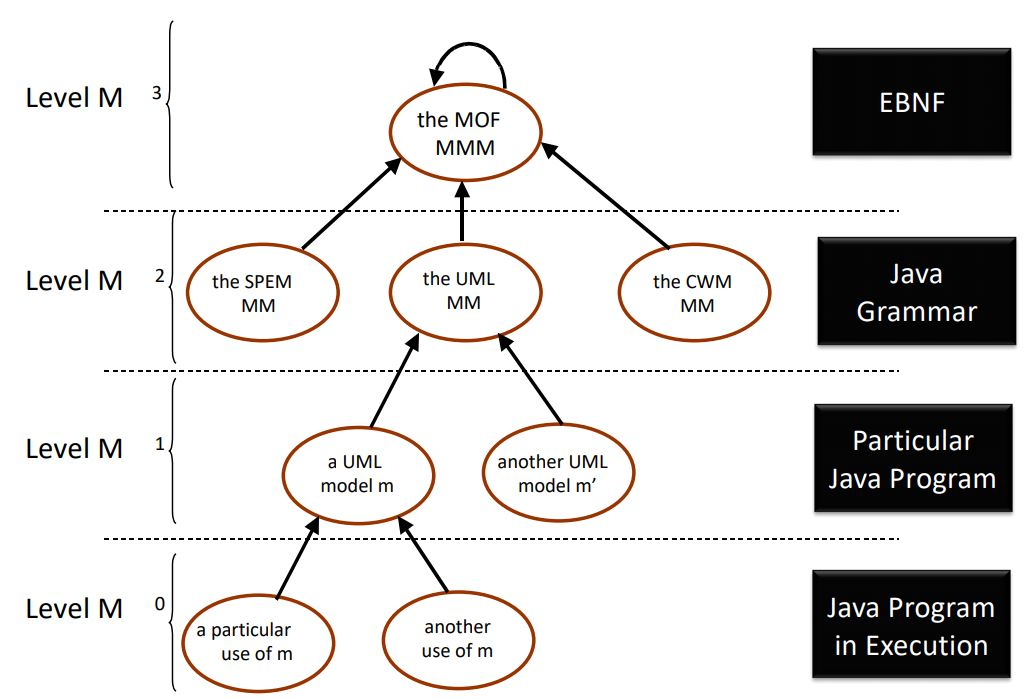
\includegraphics[scale=0.45]{res/mof-hierarchy.jpg}
			\end{figure}
		
		\pagebreak
		
		\subsection{Unified Modeling Language (UML)}
			UML is central for MDA because many tools are based on UML and its extension capabilities (UML Profiles). From version 2.0 on, UML is formally defined via the	MOF.
			
			\subsubsection{Extending UML}
				UML can not be complete, because it's not feasible to specify every details. There are two ways to extend UML/MOF: 
				\begin{enumerate}
					\item Heavyweight: completely new meta-model based on MOF (Not automatically supported by modeling tools); essentially creating a new modeling language from MOF
					\item Lightweight: Extension based on the UML Metamodel or with UML Profiles
				\end{enumerate}
				\begin{figure}[h!]
					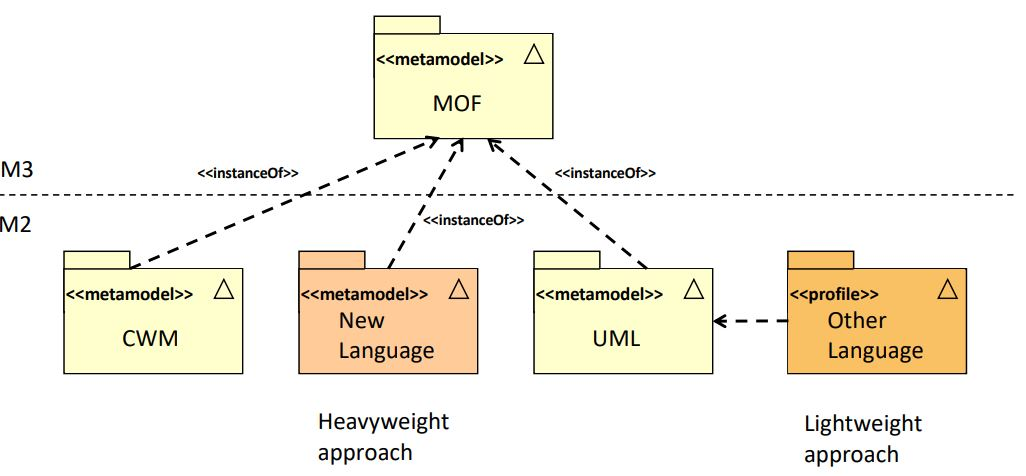
\includegraphics[scale=0.5]{res/mof-extension-methods}
					\caption{Comparison of the two extension approaches}
				\end{figure}
				
			\subsubsection{Extension based on the metamodel}
				\begin{figure}[h!]
					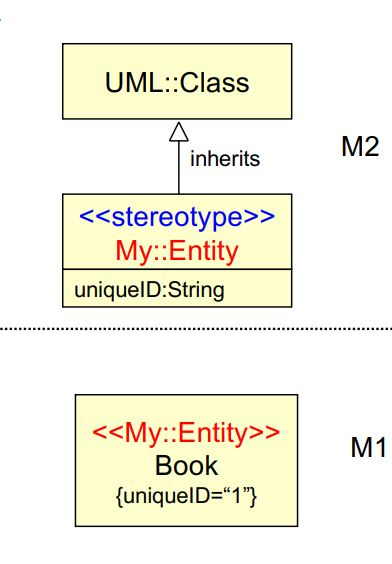
\includegraphics[scale=0.3]{res/uml-extension-metamodel.jpg}
				\end{figure}
				Two new features (can be interpreted by code generators!!!!1!!1!!!):
				\begin{itemize}
					\item Stereotype: represented by <<\ldots>>; Specifies the metaclass
					\item Tagged Value: represented by \{\ldots\}; Specifies an attribute of the metaclass
				\end{itemize}
				
			\subsubsection{UML Profiles}
				Mostly used to specialize UML for specific domains, when there is no need to change UML metamodel and semantics. They are an excellent mechanism for defining MDA 'Platforms'. A UML profile consists of:
				\begin{itemize}
					\item Stereotypes: Used to refine meta-classes (or other stereotypes) by defining supplemental semantics
					\item Tagged values: Attributes of stereotypes with user-defined semantics; Rendered as tagged values in the model in which the	stereotype is used 	
					\item OCL constraints: Predicates (e.g., OCL expressions) that reduce semantic variation; Can be attached to any meta-class or stereotype
				\end{itemize}
				There is a UML language construct for an extension: a filled inheritance arrow.\\
				An extension conforming to the UML standard must not violate the standard UML semantics
				\begin{figure}[h!]
					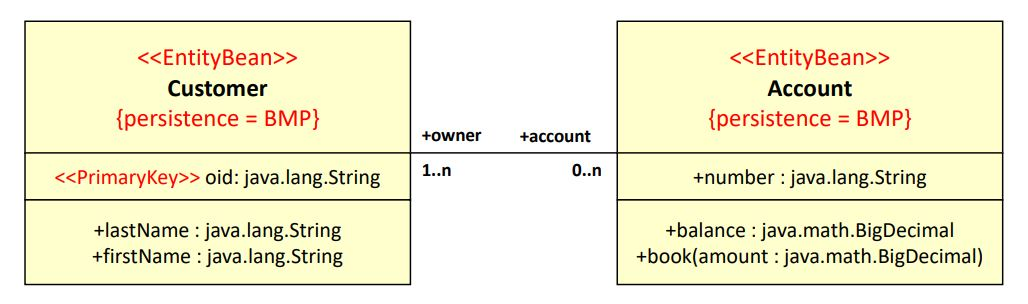
\includegraphics[scale=0.5]{res/uml-profile-ejb.jpg}
					\caption{Usage of the EJB profile}
				\end{figure}

			
			
				
				

		
		
		
		
		
		
		
		
		
		
		
		
		
		
		
		
		
		
			